\section{Introduction}
\label{sec:intro}

With the recent advances of deep learning, integrating the main modules of automatic speech recognition (ASR) such as acoustic model, pronunciation lexicon, and language model into a single end-to-end model is highly attractive. Connectionist Temporal Classification (CTC) \cite{graves2006connectionist} lends itself on such end-to-end approaches by introducing an additional blank symbol and specifically-designed loss function optimizing to generate the correct character sequences from the speech signal directly, without framewise phoneme alignment in advance. With many recent results \cite{hannun2014deep, amodei2016deep, collobert2016wav2letter}, end-to-end deep learning has created a larger interest in the speech community.

However, the end-to-end ASR system requires a huge amount of paired speech-transcription data, which is costly. 
For most languages in the world, they lack sufficient paired data for training. 
Pretraining on other language sources as the initialization, then fine-tuning on target language is the dominant approach in such low-resource settings, also known as multilingual transfer learning / pretraining (MultiASR) \cite{vu2014multilingual, tong2017investigation}. 
The backbone of MultiASR is a multitask model with shared hidden layers (encoder), and many language-specific heads. 
The model structure is designed to learn an encoder to extract language-independent representations to build a better acoustic model from many source languages. 
The success of ``language-independent'' features to improve ASR performance compared to monolingual training has been shown in many recent works \cite{cho2018multilingual, dalmia2018sequence}.

\begin{figure}[htb]

\begin{minipage}[b]{0.48\linewidth}
  \centering
  \centerline{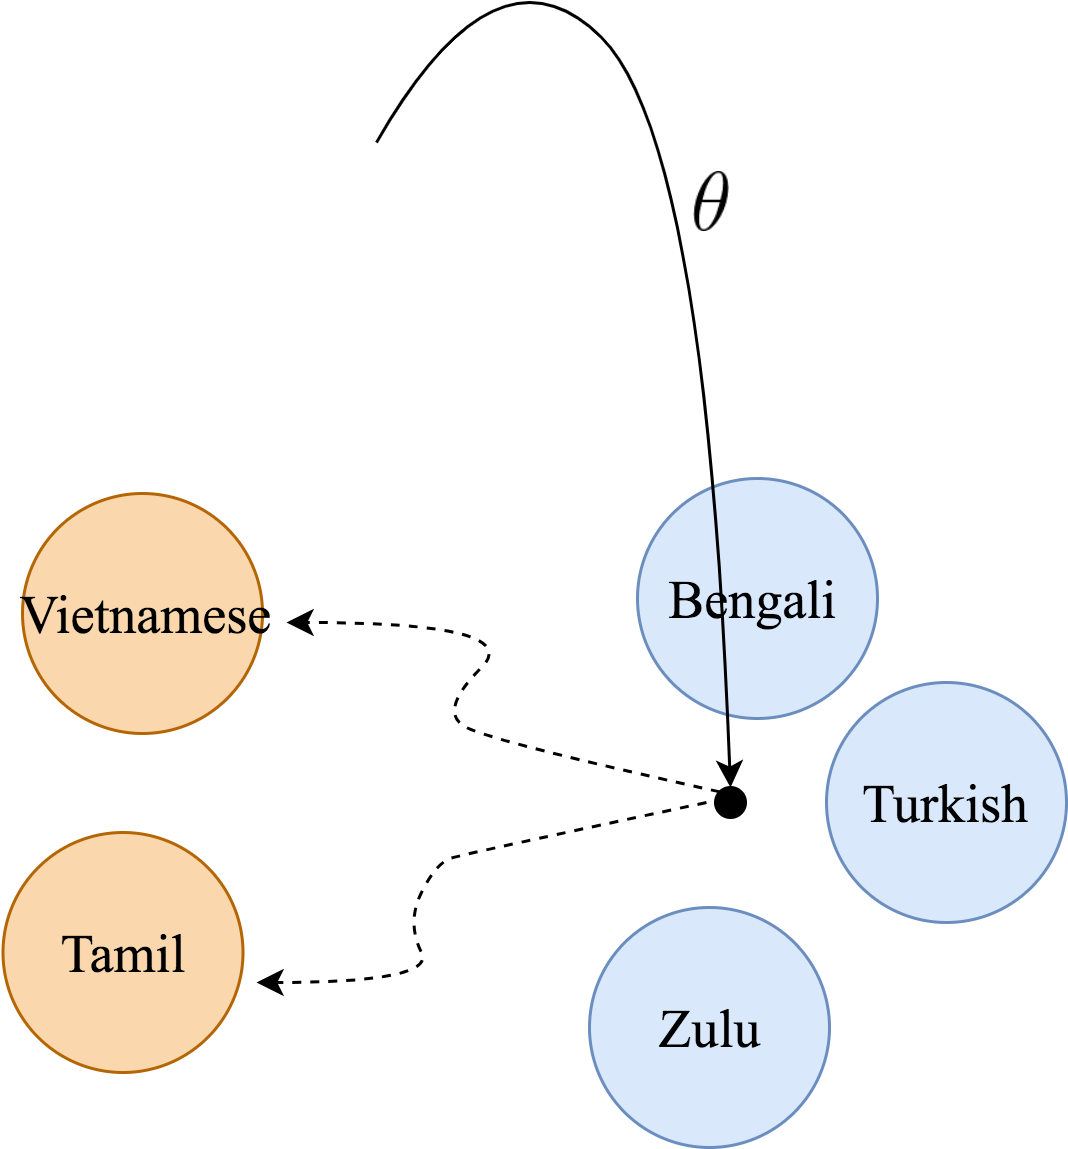
\includegraphics[width=4.0cm]{figs/multi_process.png}}
%  \vspace{1.5cm}
  \centerline{(a) MultiASR}\medskip
\end{minipage}
\hfill
\begin{minipage}[b]{0.48\linewidth}
  \centering
  \centerline{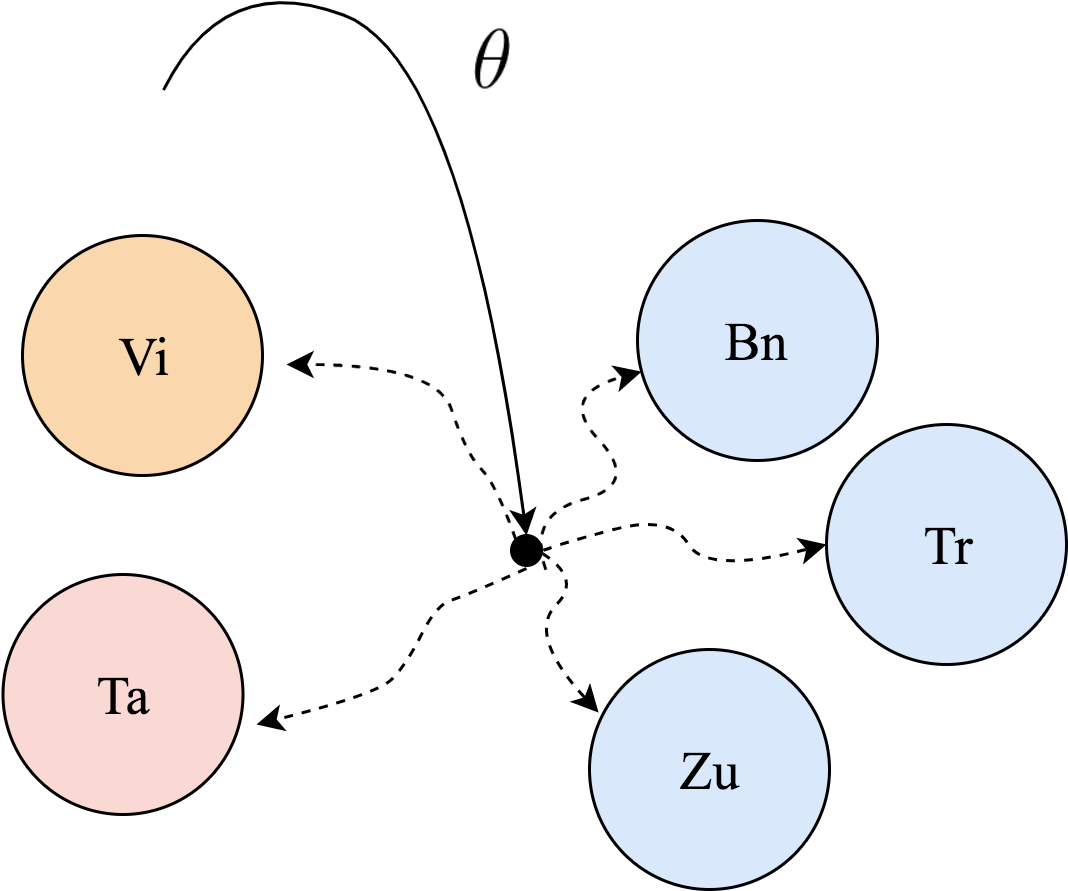
\includegraphics[width=4.0cm]{figs/meta_process.png}}
%  \vspace{1.5cm}
  \centerline{(b) MetaASR}\medskip
\end{minipage}
%
\caption{Illustration: Difference of the learned parameters from MultiASR \& MetaASR. The solid lines represent the learning process of pretraining, either multitask or meta learning. The dashed lines represent the language-specific adaptation.\\ (The figure is modified from \cite{gu2018meta})}
\label{fig:meta-idea}
%
\end{figure}



Besides directly training the model with all the source languages, there are various variants of MultiASR approaches. 
Language-adversarial training approaches \cite{Yi2018AdversarialMT, adams2019massively} introduce language-adversarial classification objective to the shared encoder, negating the gradients backpropagated from the language classifier to encourage the encoder to extract more language-independent representations. 
Hierarchical approaches \cite{Sanabria2018HierarchicalMT} introduce different granularity objectives by combining both character and phoneme prediction at different levels of the model.

%Lee: 我暫時把兩段合併,這邊應該要提到說,我們用的方法是 MAML ,可以跟任何 network architecture 結合
In this paper, we provide a novel research direction following up on the idea of multilingual pretraining -- \textbf{Meta learning}. 
Meta learning, or learning-to-learn, has recently received considerable interest in the machine learning community. The goal of meta learning is to solve the problem of ``fast adaptation on unseen data'', which is aligned with our low-resource setting.
 With its success in computer vision under the few-shot learning setting~\cite{rusu2018meta, snell2017prototypical, vinyals2016matching}, there have been some works in language and speech processing, for instance, language transfer in neural machine translation \cite{gu2018meta}, dialogue generation \cite{mi2019meta}, and speaker adaptive training \cite{klejch2018learning}, but not multilingual pretraining for speech recognition.

We use model-agnostic meta-learning algorithm (MAML) \cite{finn2017model} in this work. 
As its name suggested, MAML can be applied to any network architecture. 
MAML only modifies the optimization process following meta learning training scheme.
It does not introduce additional modules like adversarial training or requires phoneme level annotation (usually through lexicon) like hierarchical approaches. 
We evaluated the effectiveness of the proposed meta learning algorithm, MetaASR, on the IARPA BABEL dataset \cite{gales2014speech}. Our experiments reveal that MetaASR outperforms MultiASR significantly across all target languages.